\part{Applications}

\section{Electrical circuits}
	Consider the following linear circuit ($U_{input}=U,\ R_1,\ R_2$ given). Since the circuit is grounded: $U_{ground} = 0$
	\begin{center}
		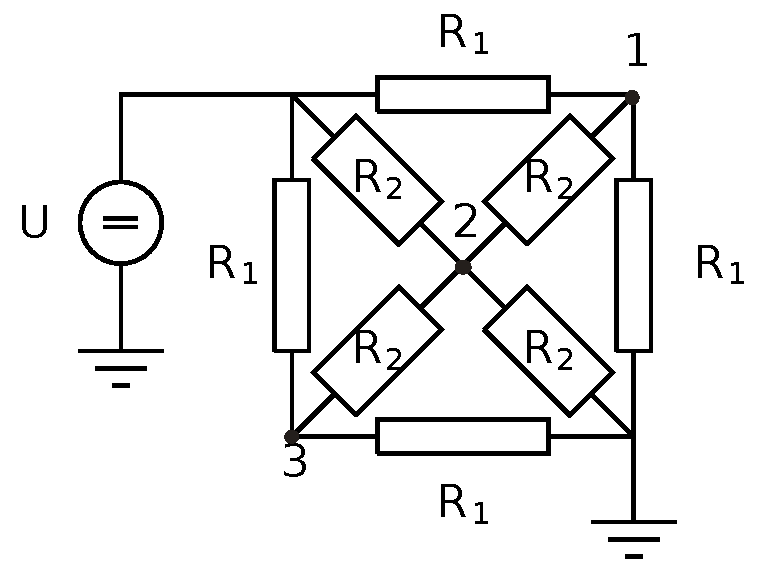
\includegraphics[width=5cm]{images/circuit1.pdf}
	\end{center}
	To derive the linear system of equations. One has to look at the specific nodes and create an LSE:
	\paragraph{Node 1}
		\begin{align*}
			\frac{1}{R_1}\cdot (U_1 - U) + \frac{1}{R_1}\cdot(U_1-0) + \frac{1}{R_2}\cdot(U_1 - U_2) &= 0\\
			\Longrightarrow \qquad \left(2 \frac{1}{R_1}+\frac{1}{R_2}\right)\cdot U_1 - \frac{1}{R_2} \cdot U_2 &= \frac{1}{R_1} \cdot U
		\end{align*}
	\paragraph{Node 2}
		\begin{align*}
			-\frac{1}{R_2}\cdot U_1 + 4 \frac{1}{R_2}\cdot U_2 - \frac{1}{R_2}\cdot U_3  = \frac{1}{R_2}\cdot U
		\end{align*}
	\paragraph{Node 3}
		\begin{align*}
			-\frac{1}{R_2}\cdot U_2 +\left(2 \frac{1}{R_1}+\frac{1}{R_2}\right)\cdot U_3 = \frac{1}{R_1}\cdot U
		\end{align*}
	Now we are able to create the LSE:
	\begin{align*}
		\begin{pmatrix}
			2 \tfrac{1}{R_1}+\tfrac{1}{R_2} & -\tfrac{1}{R_2} & 0\\
			-\tfrac{1}{R_2} & 4 \tfrac{1}{R_2} & - \tfrac{1}{R_2}\\
			0 & - \tfrac{1}{R_2} & 2 \tfrac{1}{R_1}+ \tfrac{1}{R_2}
		\end{pmatrix}
		\begin{pmatrix}
			U_1\\
			U_2\\
			U_3
		\end{pmatrix} =
		\begin{pmatrix}
			\tfrac{1}{R_1} U\\
			\tfrac{1}{R_2} U\\
			\tfrac{1}{R_1}U
		\end{pmatrix}
	\end{align*}
	
%%% Kapitel 3